\section{The Liquid Xenon Scintillating Cell (LXSC)}
\label{sec.lxsc}

\begin{figure}[!htb]
	\centering
	
	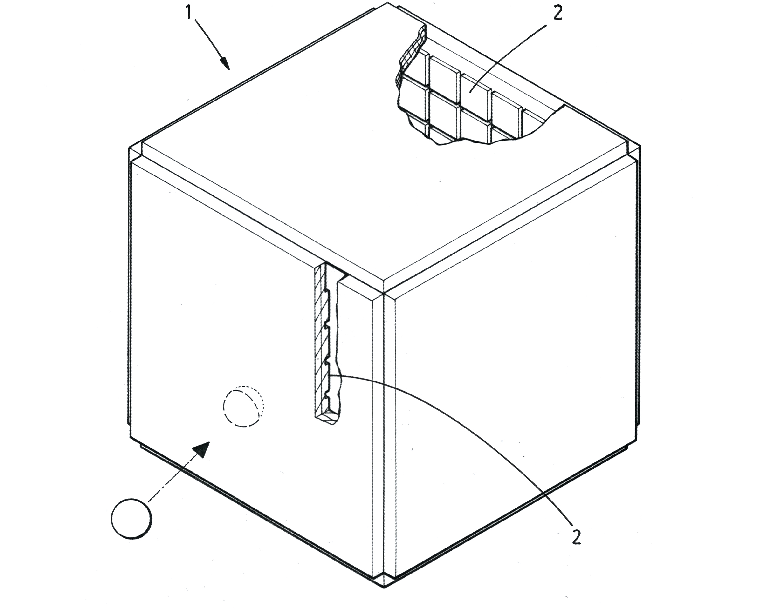
\includegraphics[scale=0.7]{img/LXSC2.pdf}
	%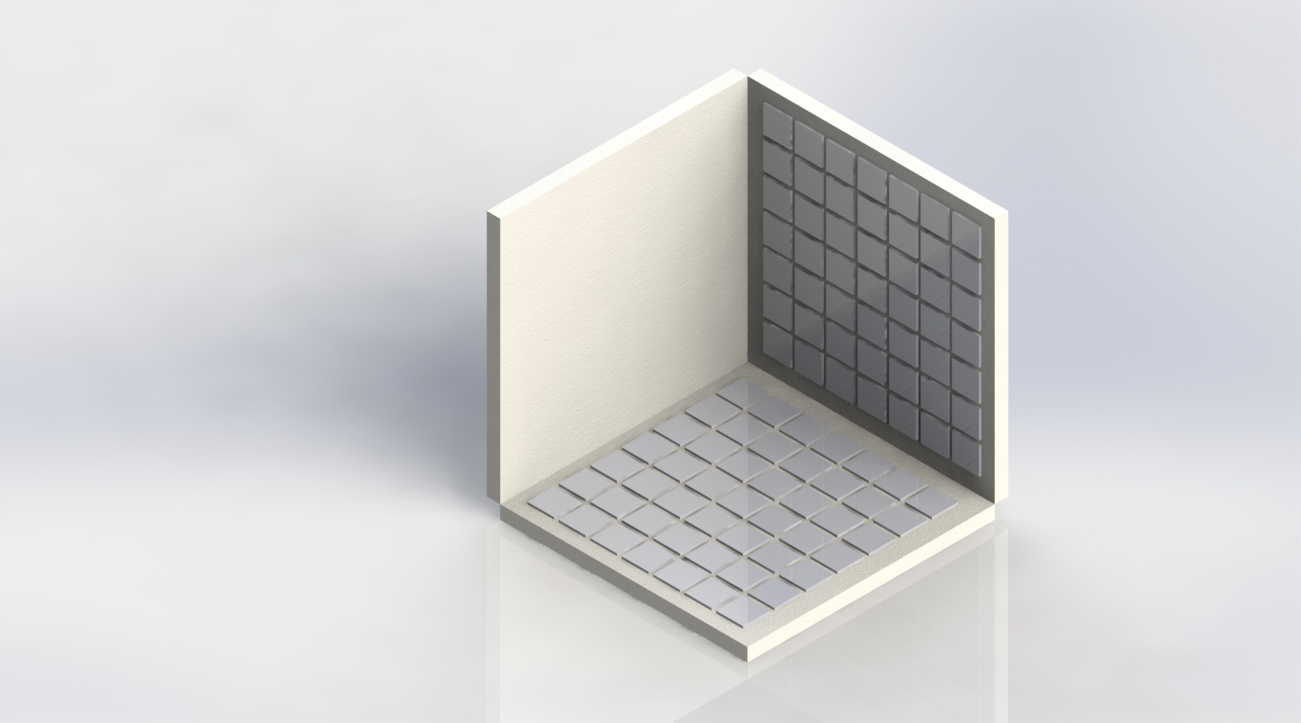
\includegraphics[scale=0.35]{img/box5open.jpg}
	\caption{\label{fig.box} The default design of the LXSC (called LXSC2) instruments the entry and exit faces of the box with large silicon photomultipliers (SiPMs), coated with a wavelength shifter, tetraphenyl butadiene (TPB). The non-instrumented faces are covered by reflecting Teflon coated with TPB.  }
\end{figure}

Figure \ref{fig.box}~shows a conceptual drawing of the keystone of the PETALO apparatus, the Liquid Xenon Scintillating Cell (LXSC). The cell is a box  filled with LXe whose transverse dimensions are chosen to optimize packing and with a thickness optimized to contain a large fraction of the incoming photons. The entry and exit faces of the box (relative to the incoming gammas direction) are instrumented with large silicon photomultipliers (SiPMs), coated with a wavelength shifter, tetraphenyl butadiene (TPB). The non-instrumented faces are covered by reflecting Teflon coated with TPB. 

%The transverse dimensions depend on the application (e.g, the diameter of the PET scanner). The default chosen for this study is of $5\times 5$ cm$^2$. The longitudinal dimension is chosen so that most of the incoming 511 keV photons interact in the volume. The default dimension is 5 cm, which results in 77\% of the initial gammas interacting in the cell. 

%The best performance from the point of view of energy resolution is obtained when all the box faces are instrumented with SiPMs, as illustrated in the left panel of Figure \ref{fig.box}. We denote this configuration as LXSC6. On the other hand, the most economical configuration is obtained instrumenting only the entry and exit faces (relative to the beam direction). We call this configuration LXSC2. Other possible configurations instrument three faces (entry, exit and one of the lateral faces, LXSC3) or four faces (entry, exit and two opposite laterals, LXSC4). 
%The faces non instrumented are covered by reflecting teflon coated with TPB. In section \ref{sec.mc} we show that an excellent performance can be obtained even with the sparse LXSC2 configuration. 

%\newpage
%\thispagestyle{newstyle}
%\section{The performance of the LXSC}
%\label{sec.mc}
%

\subsection{Dice Boards}
\label{sec.dc}

In the LXSC the SiPMs are arranged into a {\em Dice Board}, forming a matrix.
The NEXT collaboration \cite{next} has developed DBs \cite{next13,next12} for the NEXT experiment \cite{jj14}, in particular for the tracking plane of the DEMO, NEW and NEXT-100 detectors. 

\begin{figure}[!htb]
	\centering
	\subfloat[Cuflon DB]{
		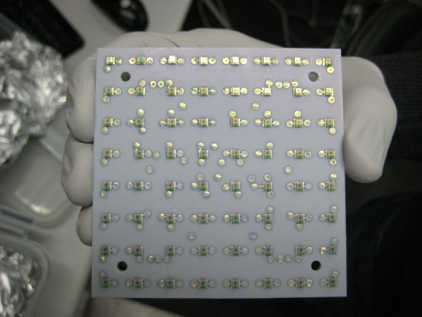
\includegraphics[width=.5\textwidth]{img/DC1.png}
		\label{fig.db1}
	}
	\subfloat[DB response to UV light]{
    	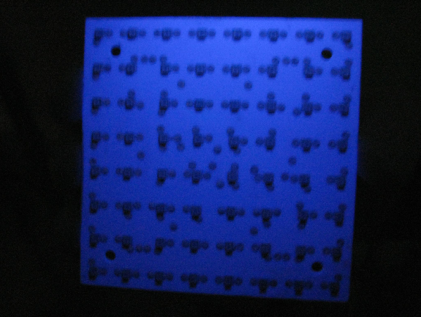
\includegraphics[width=.5\textwidth]{img/DC2.png}
		\label{fig.db2}
	}
	\caption{\label{fig.DB} Dice boards developed for NEXT-DEMO experiment. (a) DB made of Cuflon and coated with TPB. (b) Response of a DB (emitting blue light) when illuminated with a UV lamp.}
\end{figure}

Figure \ref{fig.db1} shows a DB made of Cuflon, developed for the NEXT-DEMO detector. The DB is coated with TPB, which shifts the VUV light emitted by xenon (170 nm) to blue (420 nm). Figure \ref{fig.db2} shows the response of a DB (emitting blue light) when illuminated with a UV lamp. The DBs of PETALO will have a similar design, except for the use of larger SiPMs (we are currently planning to use 6mm parts, available from several vendors).
Indeed the DBs for PETALO are easier to fabricate and much more economical than those developed for NEXT, since there are no radio purity restrictions, allowing the use of standard PCB materials such as FR4, which are forbidden in a radio pure application.

